\documentclass{beamer}
\usepackage{lipsum}
\usepackage[brazilian]{babel}
\usepackage[utf8]{inputenc}

\usepackage{enumerate}
\usepackage{dcolumn}
\usepackage{tabu}
\usepackage{colortbl}
\usepackage{booktabs}
\usepackage{changes}
\usepackage{listings}
\usepackage{placeins}
\usepackage{amsmath}

\usepackage{multirow}

\newcommand*{\Scale}[2][4]{\scalebox{#1}{$#2$}}%
\newcommand*{\Resize}[2]{\resizebox{#1}{!}{$#2$}}%

\usetheme[faculty=ppca,language=logo,framenumber,totalframenumber]{UniversiteitGent}

\title{ERLANGMS: Implantação de um barramento de serviços no CPD/UnB}
\subtitle{ \textcolor{forestgreen}{Universidade de Brasília} \\
			\textcolor{black}{Centro de Informática} \\
			3 de Maio de 2017
}
\author{Everton de Vargas Agilar \\
		E-mail: evertonagilar@unb.br
}



\begin{document}

\begin{frame}
  \titlepage
\end{frame}




%%##############################################################




\subsection{Plan}

\begin{frame}
  \frametitle{Plano}

    \begin{itemize}

	    \item<1-> Introdução
		    \begin{itemize}
		  	  \item<1-> Contexto 
		    	  \item<1-> Objetivos e Justificativa
		     \end{itemize}

		 \item<1-> Plataforma agnóstica de serviços
		    \begin{itemize}
				\item<1-> Sobre o projeto ERLANGMS
				\item<1-> Modelo baseado em atores e a linguagem ERLANG/OTP
				\item<1-> Benefícios que podem ser obtidos com o barramento
		     \end{itemize}

  	  	 \item<1-> Principais Resultados do Trabalho
		    \begin{itemize}
				\item<1-> Desenvolvimento de serviços utilizando com o SDK
				\item<1-> Autenticação de usuários com o proxy LDAP
				\item<1-> Autenticação e Autorização de serviços REST com OAuth2
  		     \end{itemize}
  	  
	   	  \item<1-> Conclusões/Trabalhos Futuros
	   	  
    \end{itemize}

\end{frame}




%%##############################################################




\section{Introdução}


\subsection{Introdução}


\begin{frame}
  \frametitle{Contexto}

  \begin{exampleblock}{Modernização de Sistemas Legados}
  
  “\textbf{Legacy information systems} are typically the
	backbone of an organization’s information flow
	and the main vehicle for consolidating business
	information. They are thus mission critical, and
	their failure can have a serious impact on
	business.” [BENNET95]

	\vspace{0.5cm} 

	“Migrate Systems Incrementally recommends that the old system be
	gradually and incrementally replaced by the new system. New
	results can then be integrated as you proceed...” [DEMEYER et al. 2002]
  \end{exampleblock}

  
\end{frame}




%%##############################################################





\begin{frame}
  \frametitle{Contexto}

  \begin{exampleblock}{Relatório de Gestão do CPD/UnB 2010-2012}
  
		“Foi identificada a necessidade de remodelação de todos os sistemas
da UnB visando uma atualização tecnológica e uma melhor
integração de seus fluxos.” ... [cpd.unb.br/transparencia]

    \begin{itemize}
  	  \item<1-> Alto custo de manutenção para manter os sistemas legados;
   	  \item<1-> Duplicação das regras de negócio entre os sistemas;
  	  \item<1-> Dificuldades para integrar os sistemas.
    \end{itemize}


  \end{exampleblock}

  
\end{frame}




\begin{frame}
  \frametitle{Objetivos}
  
    \begin{itemize}
       \item<1-> Propor uma abordagem para modernizar os sistemas legados de
forma orientada a serviços (SOA) composto por:

    \begin{itemize}
       \item<1->um barramento de serviços desenvolvido;
       \item<1->um processo de modernização para guiar os trabalhos de modernização de software; 
       \item<1->um kit de desenvolvimento (SDK) para implementar serviços independente da
       linguagem de programação.
    \end{itemize}
				
    \end{itemize}
    
\end{frame}





\begin{frame}
  \frametitle{Justificativa}
  
    \begin{itemize}
       \item<1->Maior reuso dos fluxos de negócios e maximização da
modularidade das aplicações;
       \item<1->Permitir a modernização das aplicações com menor dependência tecnológica;
       \item<1->Experimentar SOA (Service Oriented Architecture).
				
    \end{itemize}
    
\end{frame}


\subsection{Panorama geral sobre modernização na literatura}


\begin{frame}
  \frametitle{Justificativa \\ \small{Panorama geral sobre modernização na literatura}}

 	%% Mostra o diagrama de bolhas
  	
	\begin{figure}
	\centering
		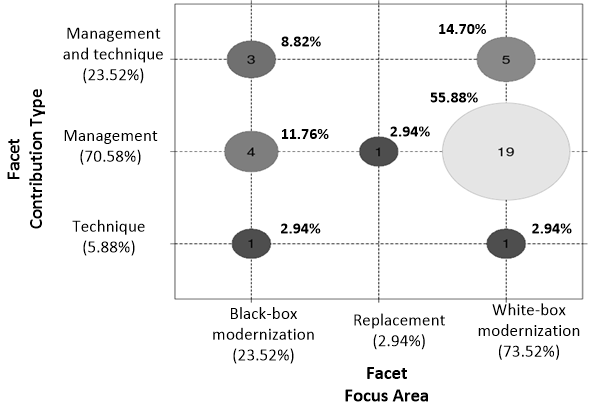
\includegraphics[scale=0.4]{img/bubble_diagram.png}
	\end{figure}
  
\end{frame}



%%##############################################################


\section{Plataforma agnóstica de serviços}


\begin{frame}[c]{ }
\centering
  \huge{Plataforma agnóstica de serviços}
\end{frame}



\subsection{Sobre}


\begin{frame}
  \frametitle{Sobre}

  \begin{exampleblock}{ERLANGMS}
  
É uma plataforma de software desenvolvida para facilitar a integração de sistemas por meio de um barramento 
de serviços multiplataforma orientado a contratos de serviços + SDK + Processo Documentado (SMSOC).

  \end{exampleblock}

  
\end{frame}


\begin{frame}
  \frametitle{Sobre}

  \begin{exampleblock}{ERLANGMS: Características do Barramento}
  
	  \begin{itemize}
		\item<1->Arquitetura Modular, multiplataforma e microserviços;
	    \item<1->Serviços são especificados em catálogos de serviços (Formato JSON);
	    \item<1->Podem haver vários nodes (ex.: Erlang nodes, JBoss Containers) formando um cluster)
	    			para evitar um ponto único de falhas;
    	    \item<1->Design RESTful;
    	    \item<1->Desenvolvimento de serviços em Erlang, Java e .Net (em progresso);
   	    \item<1->Modelo de concorrência: Actor Model;
    	    \item<1->Escalável com baixo uso de recursos e tolerante a falhas (supervisores);
    	    \item<1->Fácil compilação e instalação.
	  \end{itemize}

  \end{exampleblock}

  
\end{frame}


\begin{frame}
  \frametitle{Sobre}

  \begin{exampleblock}{ERLANGMS: Principais recursos/features}
  
	  \begin{itemize}
		\item<1->HTTP/2, HTTP/1.1, HTTPS (Secure TLS Listener);
	    \item<1->LDAP v3 -- Proxy LDAP;
	    \item<1->HTTP Basic authentication;
    	    \item<1->OAuth2 authentication (em progresso);
		\item<1->SDK para criar serviços em Java;
		\item<1->Api query padrão -- filter, fields, sort
	  \end{itemize}

  \end{exampleblock}

  
\end{frame}


\begin{frame}
  \frametitle{Sobre}

  \begin{exampleblock}{ERLANGMS: Principais recursos/features experimentais}
  
	  \begin{itemize}
		\item<1->Implementação de serviços para consulta de arquivos csv;
 	    \item<1->Implementação de serviços para consulta de dados SQL-Server;
	    \item<1->Suporte para Django template (processamento de template no back-end)
    	    \item<1->JSON Schema Draft 4 para descrever/validar a entrada/saída de dados;
	  \end{itemize}

  \end{exampleblock}

  
\end{frame}


\begin{frame}
  \frametitle{Algumas questões sobre design e arquitetura}

  \begin{exampleblock}{}
  
	  \begin{itemize}
		\item<1->(QP1) Porque o barramento foi desenvolvido com 
		uma linguagem pouco conhecida (Erlang/OTP) em vez de uma linguagem mais tradicional como C, C++ ou Java?
	    \item<1->(QP2) Porque o desenvolvimento de um novo barramento em vez de utilizar um existente?
	    \item<1->(QP3) Porque não implementar os web services usando somente Java e seus frameworks?
	  \end{itemize}
  
  \end{exampleblock}

  
\end{frame}


\begin{frame}
  \frametitle{QP1-- Porque Erlang OTP}

    \begin{itemize}
       \item<1-> Suporta aplicações distribuídas e tolerantes a falhas a serem executadas em um ambiente de tempo real e ininterrupto;
       \item<1-> Possui um ambiente de execução que realmente facilita o desenvolvimento de software de rede e de clusters de serviços;
       
       \item<1-> Possui um modelo de arquitetura baseado em atores (Actor Model) onde os processos podem 
       se comunicar apenas por mensagens;
       
    \end{itemize}
  
\end{frame}


\begin{frame}
  \frametitle{QP1-- Quem usa Erlang OTP}

	  \begin{itemize}
		\item<1->Facebook, no backend de seu sistema de chat, lidando com 100 milhõs de usuários ativos e
		Whatapps, nos servidores de mensageria, lidando com 2 milhões de usuários conectados por servidor;
		\item<1->Yahoo em seu serviço de bookmark, Delicious, que tem mais de 5 milhões de usuários e mais de 150 milhões de bookmarks;
		\item<1->Amazon SimpleDB, o serviço de dados do Amazon EC2;
		\item<1->GitHub, no seu sistema de backend, lidando com milhares de transações concorrentes;
		\item<1->T-Mobile nos seus sistemas de SMS e autenticação;
		\item<1->Motorola, CouchDB, RabbitMQ, Ejabbed, entre outros.
						
	   \end{itemize}
  
\end{frame}


%%##############################################################






%%##############################################################


\subsection{Perguntas}


\begin{frame}[c]{ }
\centering
  \huge{Perguntas ?}
\end{frame}



\end{document}



